\section{Numerical experiments}
\label{ch7:sect:exp}
In this section, we implement the strategies described in Section~\ref{ch7:sect:methodology} on two case studies, namely the 2D airfoil inverse design (Section~\ref{ch7:sect:AirfoilCase}) and 3D wing inverse design (Section~\ref{ch7:sect:wingCase}).

\subsection{2D airfoil inverse design case}
\label{ch7:sect:AirfoilCase}
In this particular case, the generative inverse design process is required to propose airfoil candidates that satisfy the lift coefficient $C_{L} = 0.7$ when the Mach number $M=0.2$, angle of attack $\alpha=2^\circ$, and Reynolds number $Re = 1\times10^{6}$. We use \texttt{NeuralFoil}\footnote{\texttt{NeuralFoil} repository: \url{https://github.com/peterdsharpe/NeuralFoil} (last accessed on 22 July 2025)} as surrogate model for rapid airfoil aerodynamic analysis. \texttt{NeuralFoil} is implemented as a hybrid of analytical models and neural networks trained on tens of millions of \texttt{XFoil}\footnote{XFoil webpage: \url{https://web.mit.edu/drela/Public/web/xfoil/} (last accessed on 22 July 2025)} runs. \texttt{NeuralFoil} supports auto-differentiation and has been proven effective on various gradient-based design optimization cases~\cite{aa.Sharpe2024}. The CST method~\cite{aa.Kulfan2008} is used for the airfoil shape parameterization. The airfoil geometry is controlled by a total of 16 parameters, with eight shape coefficients assigned to the upper surface and the other eight to the lower surface. 

\subsubsection{Guidance controllability}
\label{ch7:subsect:physicalloss}
Here, we investigate the guidance controllability; we first investigate the $\mathcal{L}_{\mathrm{phys}}$ curve and precision achieved by the four strategies shown in Figure~\ref{ch7:fig:fmStrategy} (Section~\ref{ch7:subsect:physics}). All quantitative results of model performance are provided in Table~\ref{ch7:tab:modelPerformanceResults} in Appendix~\ref{ch7:subsect:modelPerformance}. The discussion below is focused on the results obtained using the energy-based approach.

For the energy-based approach, we generate $200$ samples with $\lambda = 10$ under different physics injection cutoff times ($t_c = 0.0, 0.2, 0.6, 0.8$) and total inference time steps ($T = 200, 1000, 2000$). Figure~\ref{ch7:fig:mean_loss_curve_1k} shows the loss decay curve when $T=1000$. 
\begin{figure}[htbp]
    \centering
    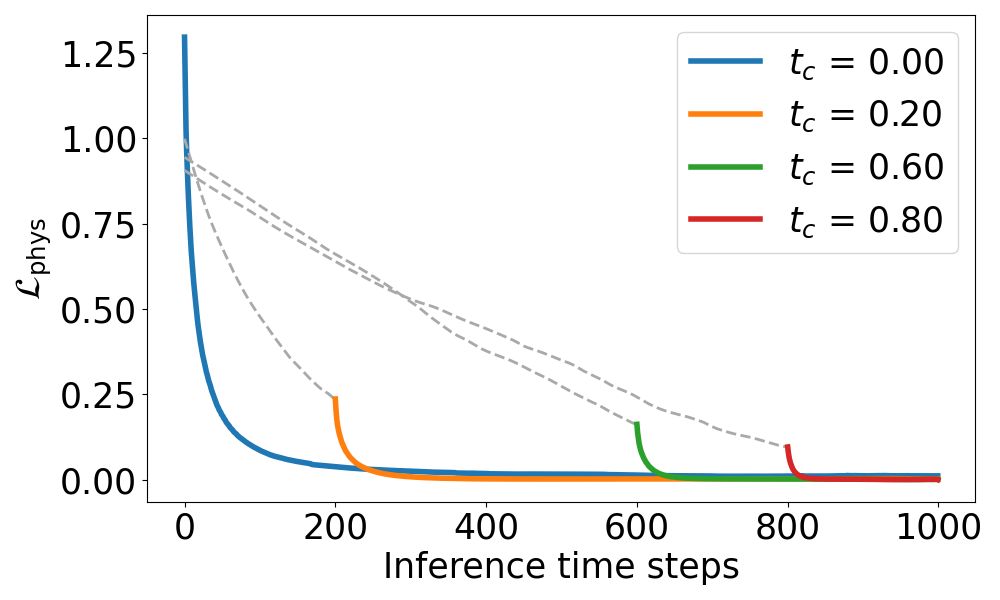
\includegraphics[width=0.65\linewidth]{chapter7/fig/mean_loss_curves_all_T_1000.png}
    \caption{The mean loss curves fo energy-based approaches, when $t_c = 0.0, 0.2, 0.6, 0.8$, $T=1000$ (gray dashed lines represent \textit{pseudo‐loss} curves).}
    \label{ch7:fig:mean_loss_curve_1k}
\end{figure}
We compute the surrogate model’s \textit{pseudo‐loss} ($\mathcal{L}_{\mathrm{phys}}$ during unconditional generation) for different $t_c$ values, which are shown as gray dashed lines. These lines illustrate the $\mathcal{L}_{\mathrm{phys}}$ decay behavior under the energy-based approach's inference-physics coupling optimization process. Unconditional generation over certain inference time steps provides a good initialization by achieving a lower initial $\mathcal{L}_{\mathrm{phys}}$.

Next, we apply \textit{Dflow‐SUR} to 200 samples. Specifically, we draw 200 random initial guesses, execute the \textit{Dflow‐SUR} procedure on each sample, and record their trajectories. We then compare the performance of both the energy‐based approach and \textit{Dflow‐SUR} in terms of $\mathcal{L}_{\mathrm{phys}}$, $C_{L}$ accuracy, and inference time, which are shown in Figure~\ref{ch7:fig:modelPerformanceCompare}. Overall, compared to the energy-based method, \textit{Dflow-SUR} meets the aerodynamic constraint of $C_L = 0.7$ while driving the $\mathcal{L}_{\mathrm{phys}}$ down from $10^{-3}$ to $10^{-8}$ and achieving the shortest inference time. 

\begin{figure}[htbp]
    \centering
    \subfloat[Physical loss ($\mathcal{L}_{\mathrm{phys}}$ of final generated airfoils)\label{ch7:subfig:phys_loss}]{%
        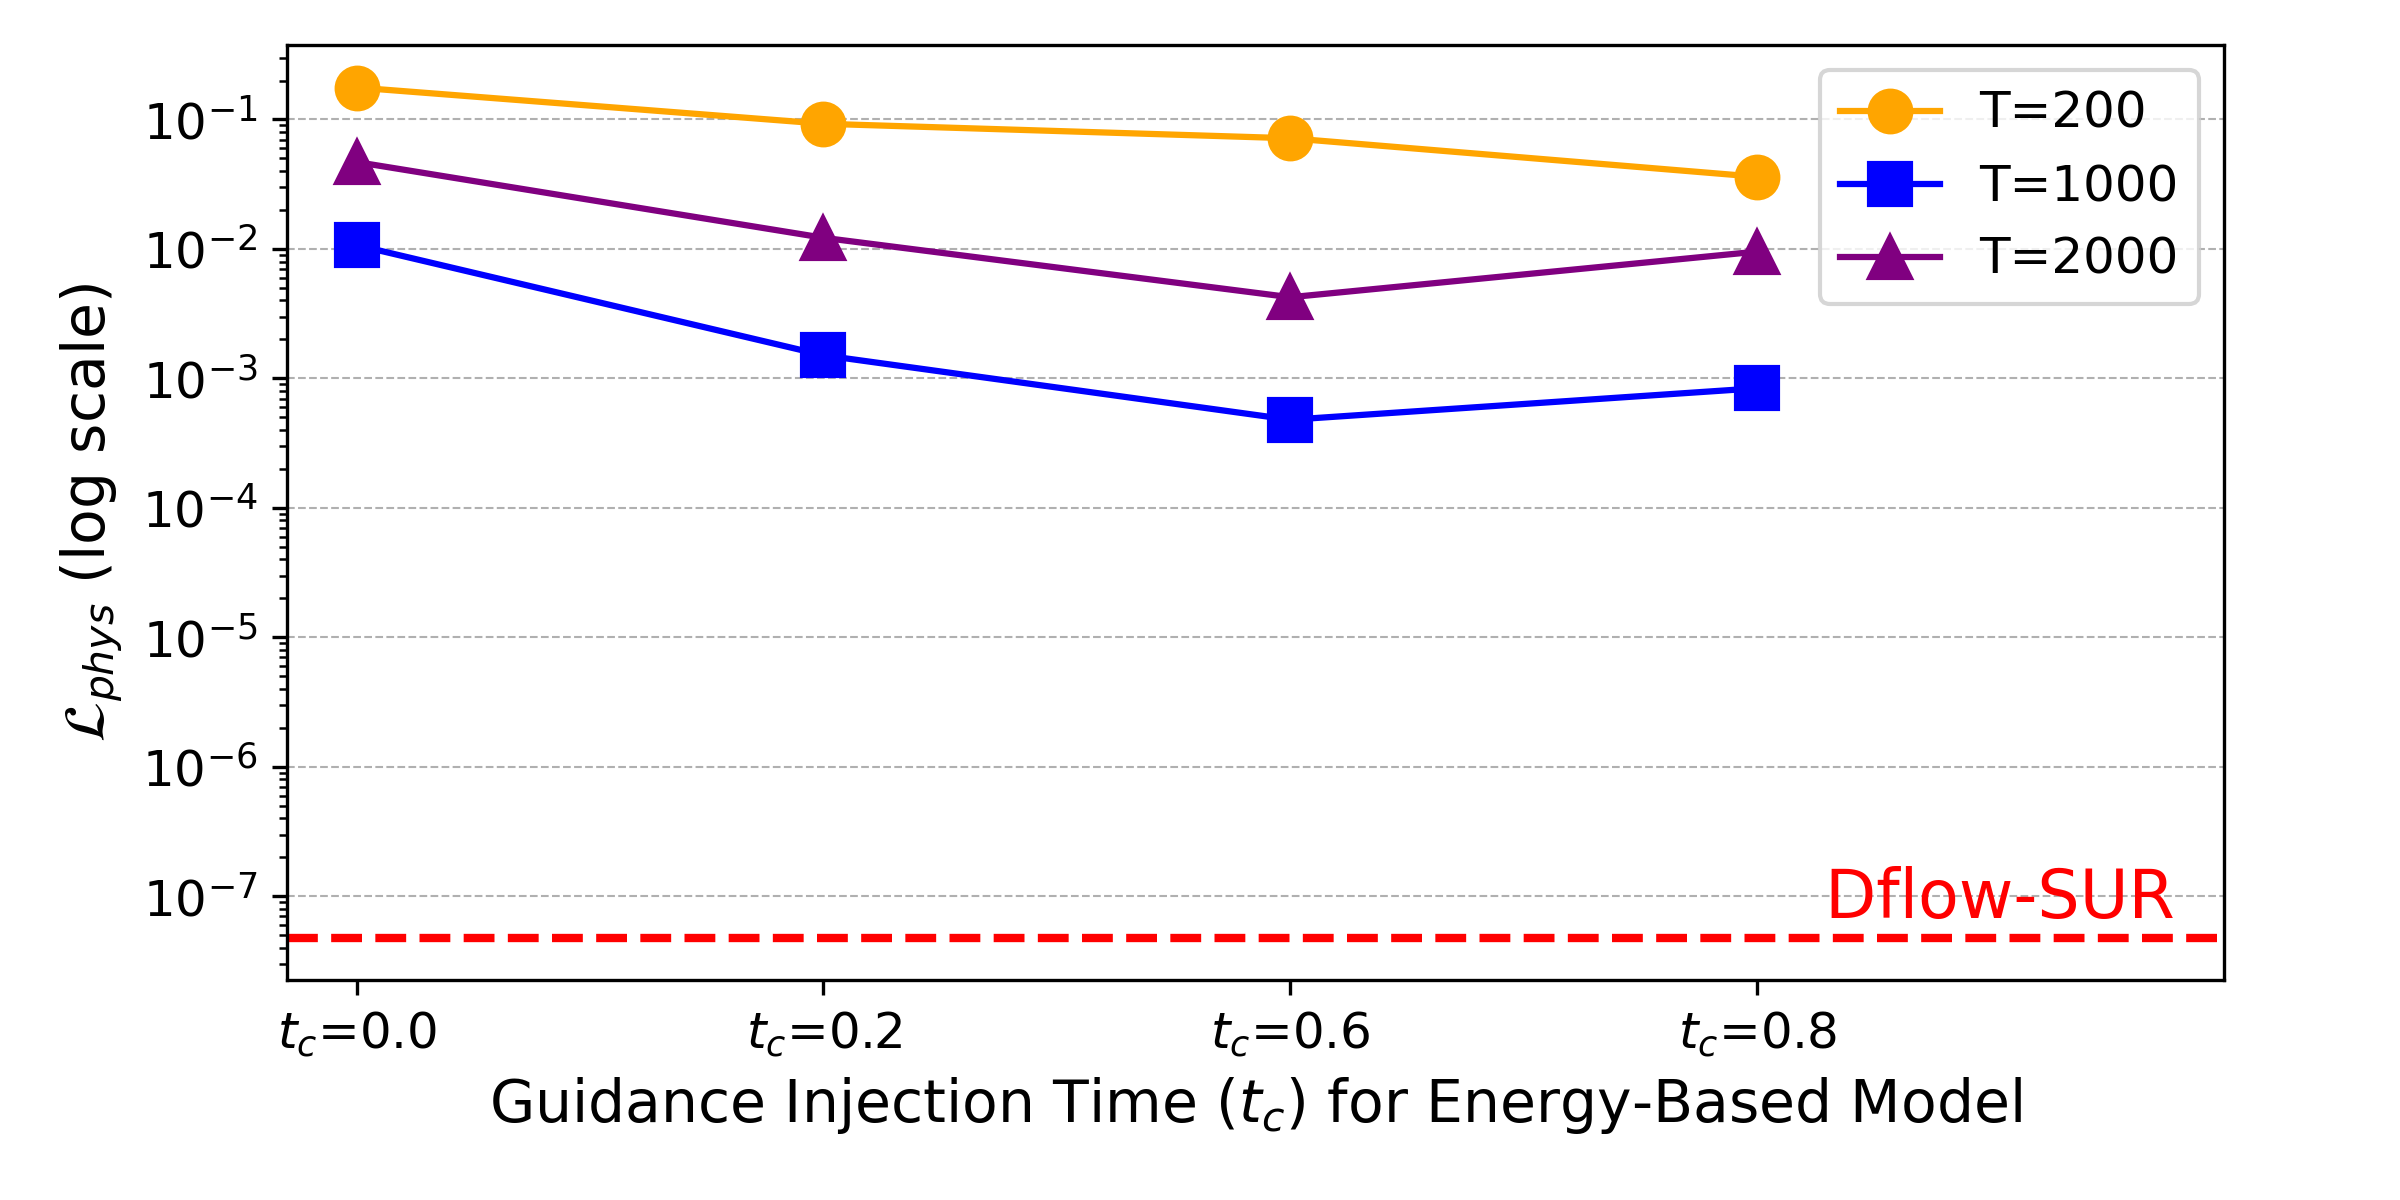
\includegraphics[width=0.8\textwidth]{chapter7/fig/physical_loss_comparison.png}%
    }\\[1em]
    \subfloat[Accuracy of lift coefficient ($C_{L}$) ($C_{L}$ of generated airfoils, with targeted $C_{L}=0.7$)\label{ch7:subfig:cl_acc}]{%
        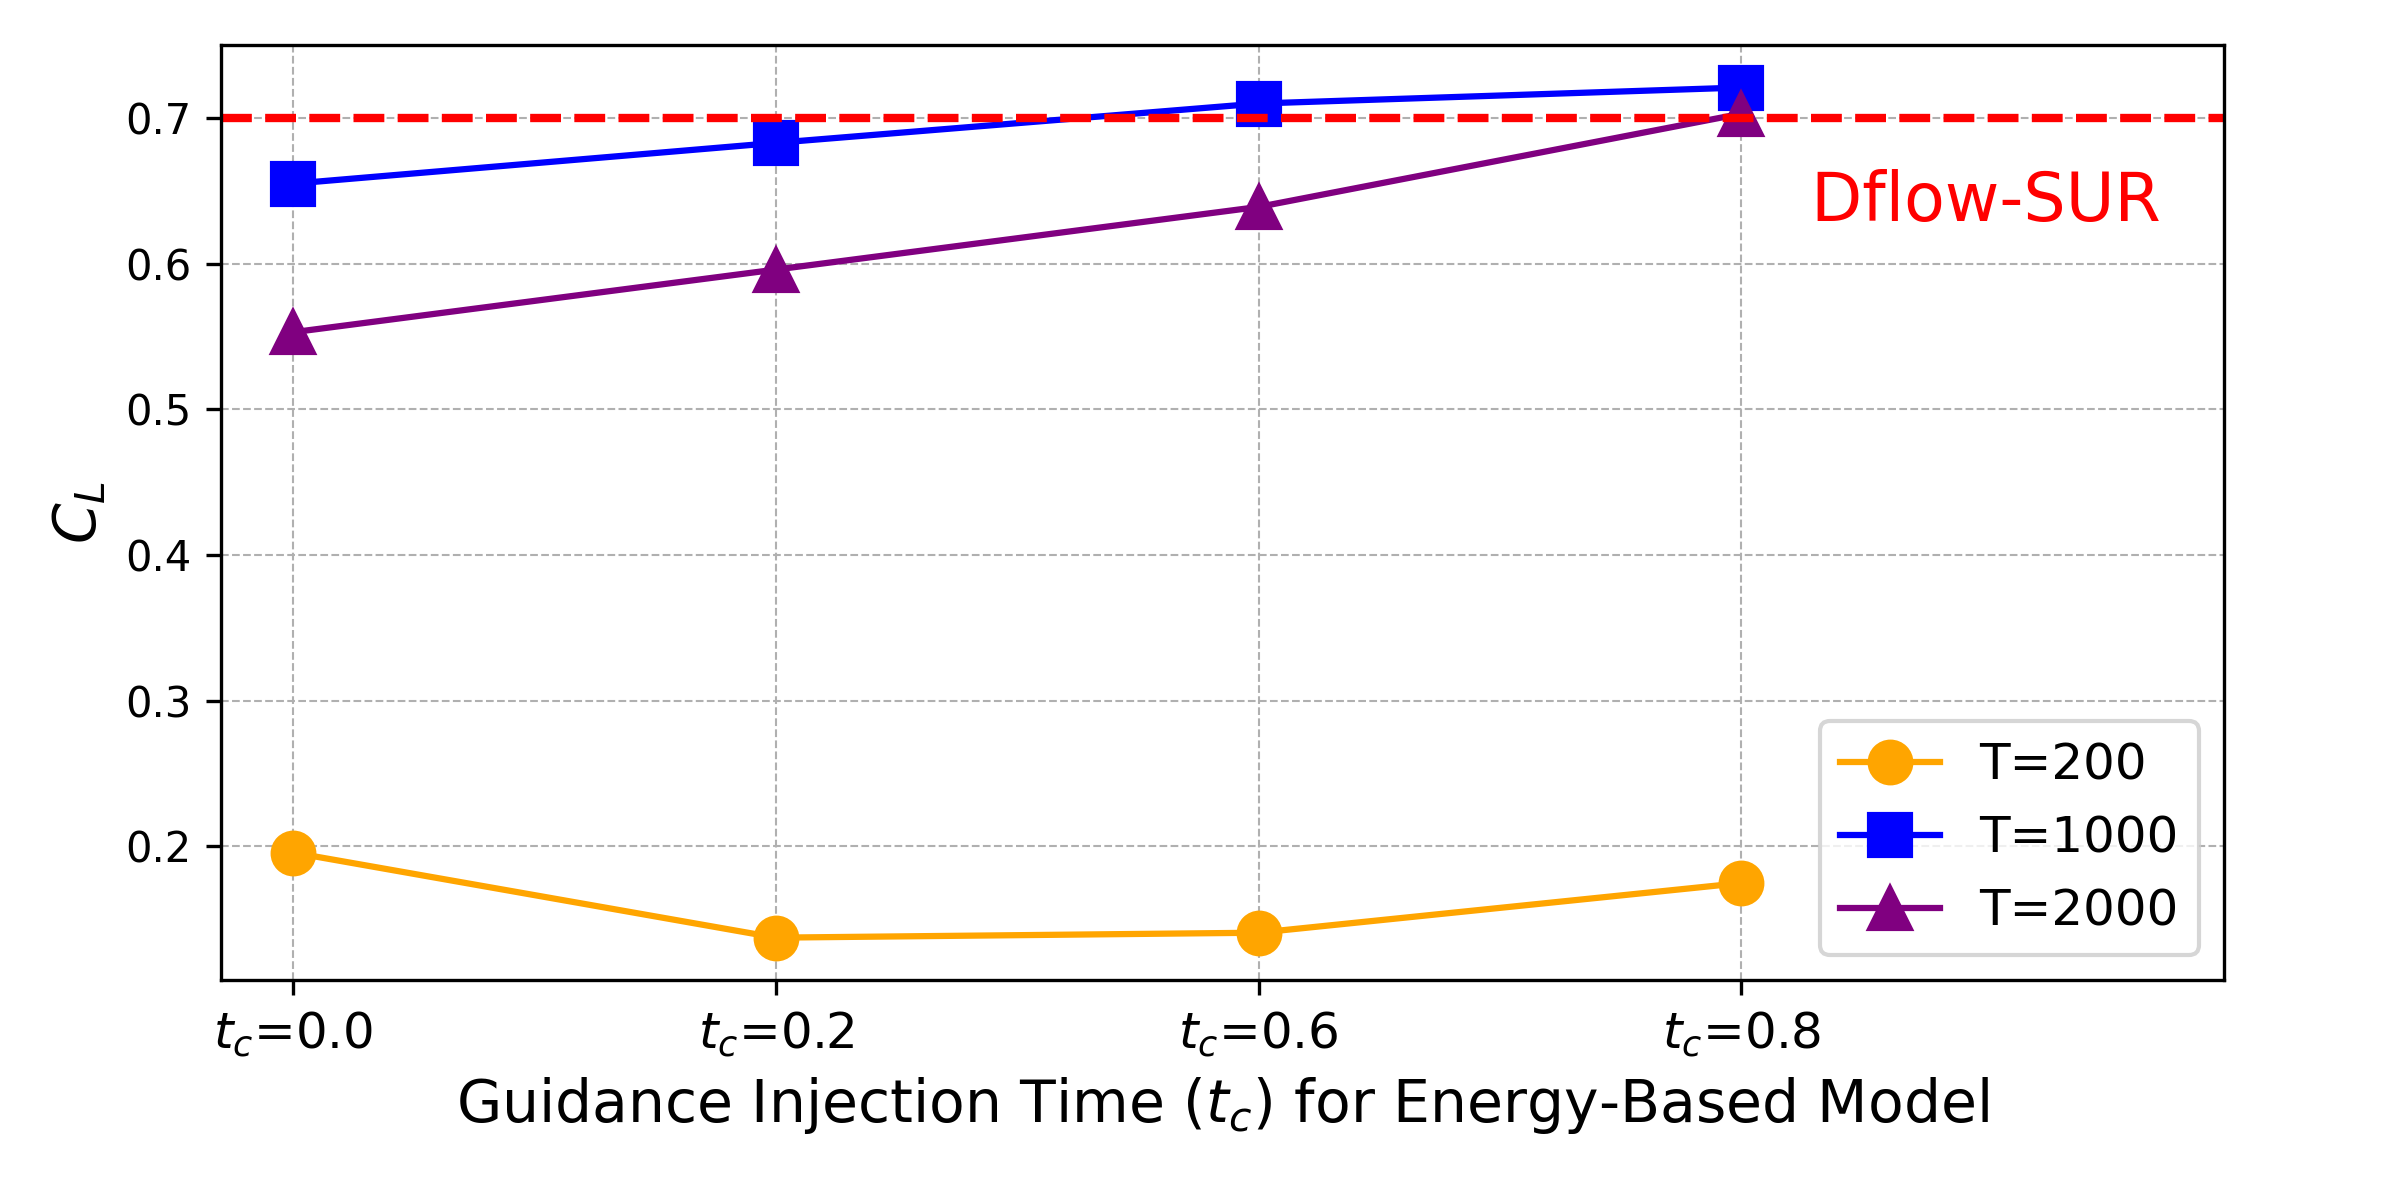
\includegraphics[width=0.8\textwidth]{chapter7/fig/cl_accuracy_comparison.png}%
    }\\[1em]
    \subfloat[Inference time\label{ch7:subfig:inf_time}]{%
        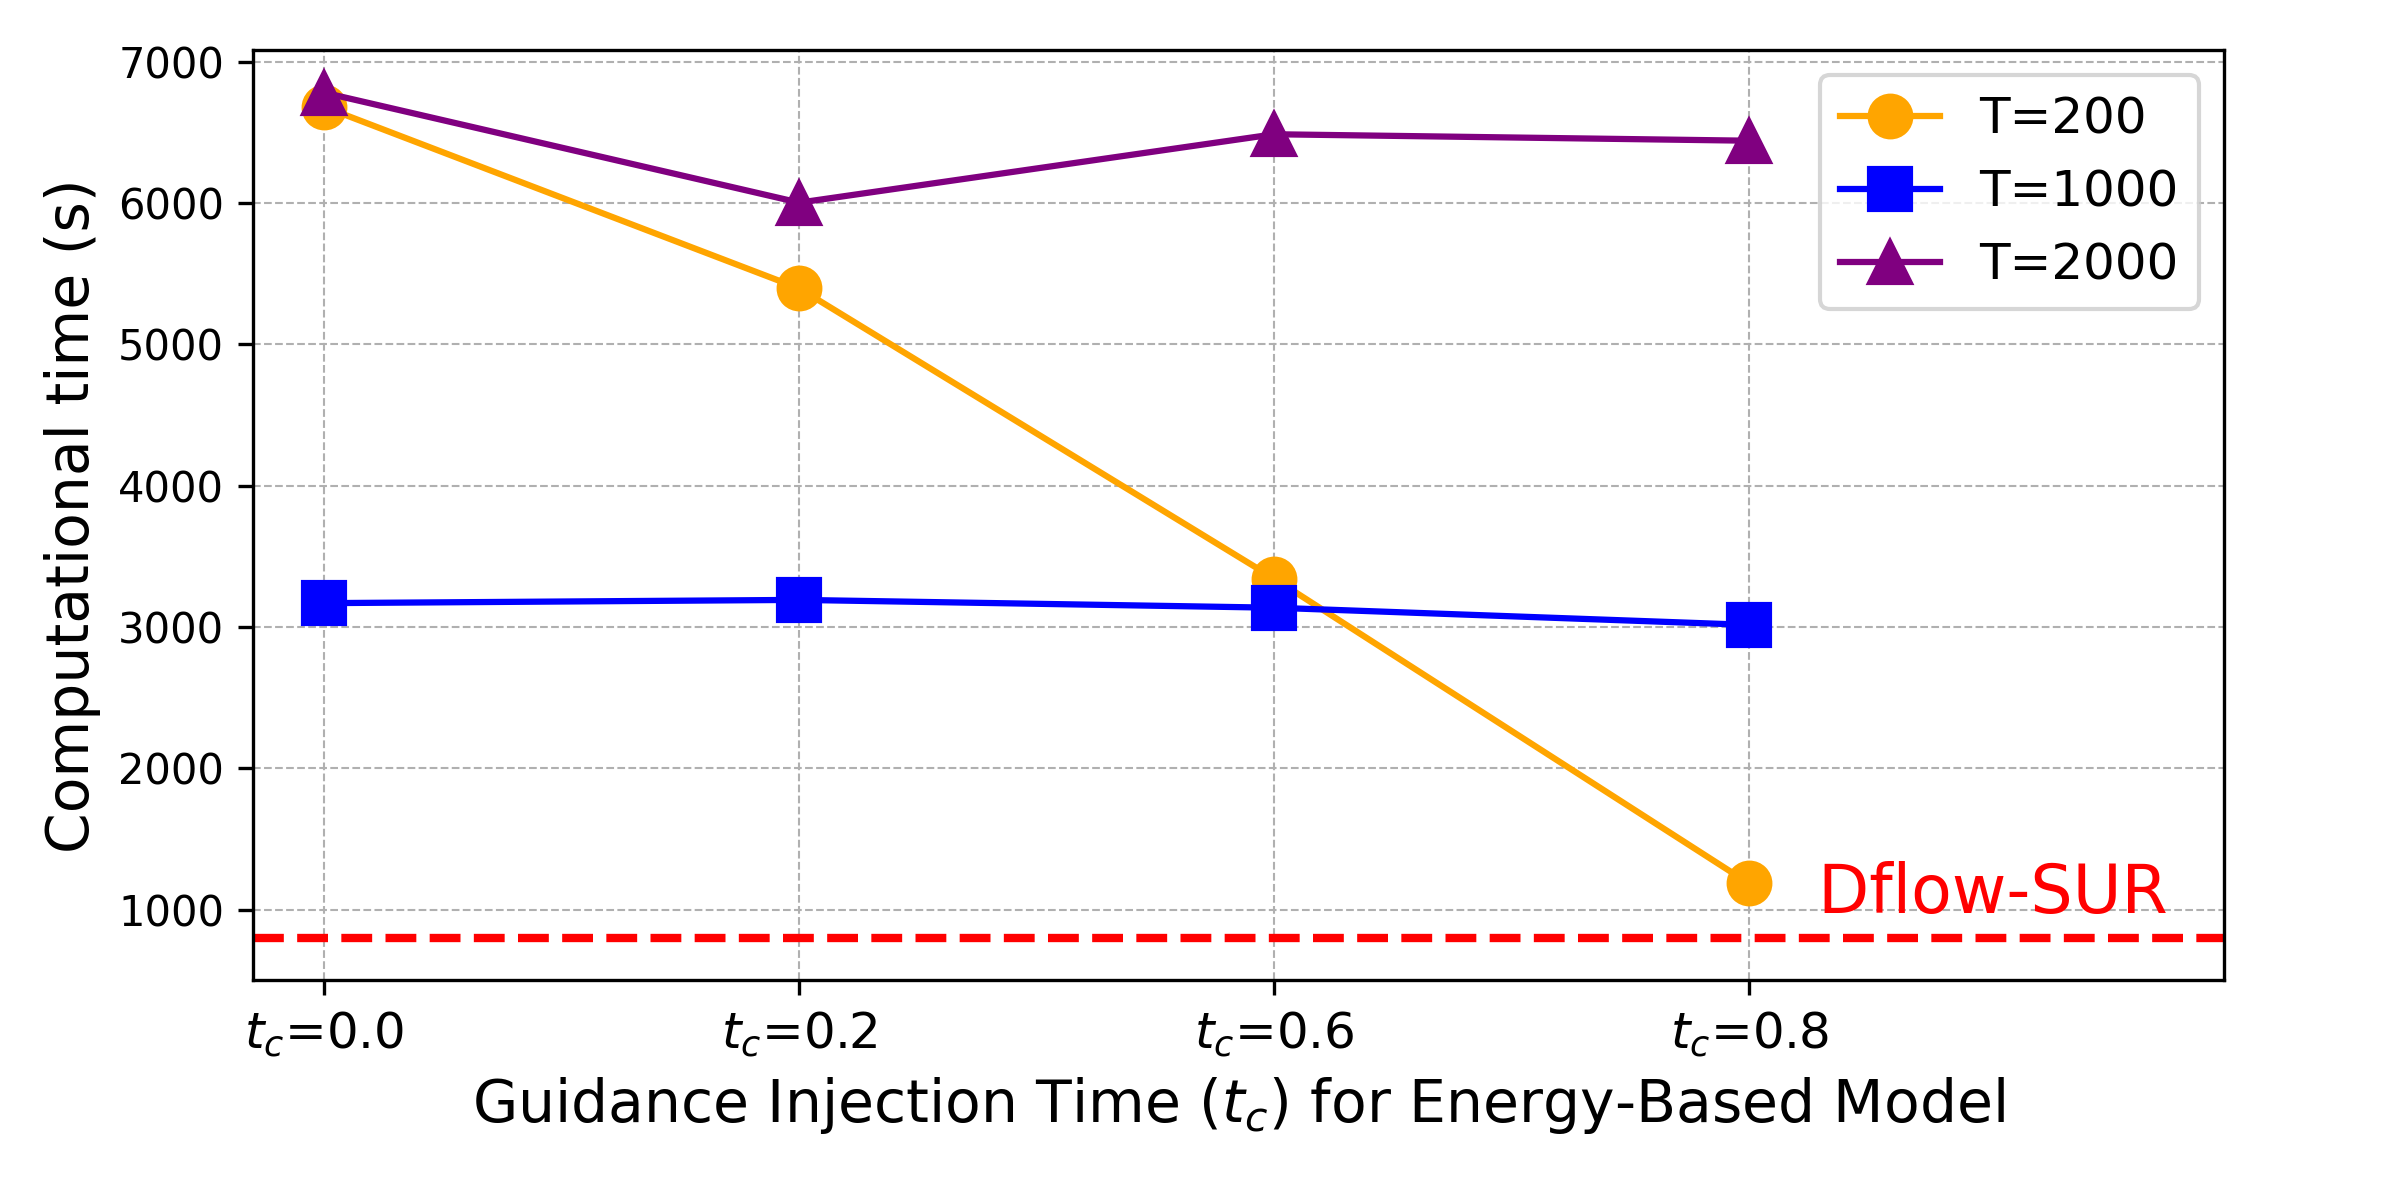
\includegraphics[width=0.8\textwidth]{chapter7/fig/inference_time_comparison.png}%
    }
    \caption{Performance comparison between the energy-based approach and \textit{Dflow‐SUR} in three metrics.}
    \label{ch7:fig:modelPerformanceCompare}
\end{figure}


This improvement arises chiefly from \textit{Dflow-SUR}’s decoupling of the inference process from the $\mathcal{L}_{\mathrm{phys}}$ optimization, which enhances gradient‐utilization efficiency compared to the tightly coupled mechanism of energy-based methods. Decoupling is effective because the inference and physics-loss objectives exhibit \textit{gradient collision} when optimized jointly. To illustrate this phenomenon in detail, we perform the following experiments. 


% In summary, based on the foregoing figures and tables, we conclude that Dflow-SUR outperforms the energy-based approach in achieving the desired physical-constraint accuracy. This lies in two aspects:

% First, compared to the Energy-based method, which injects physical losses for gradient optimization only at local intermediate time steps and thus can only correct the current local state while lacking a global perspective, Dflow-SUR formulates the physical loss $L$ as a function of the initial state $x(0)$. By leveraging the inference of the entire flow-matching velocity field $u(t)$ (as described in Equation 1), Dflow-SUR avoids interference from truncation errors and is capable of capturing global interaction relationships across temporal steps.

% Another reason is that DFlow-SUR consistently maintains generation on the data manifold, which not only ensures the uncertainty quantification by the surrogate model but also guarantees the numerical stability and solution accuracy of the solver. Recent studies have demonstrated that incorporating energy guidance in diffusion or flow generation leads to samples deviating from the data manifold, thereby inducing an irreducible lower bound of the guided estimation error. This \textit{Manifold shift} recurs at each time step, causing the error to gradually amplify. We will further discuss this problem in Section~\ref{ch7:subsect:uncertainty}.


Referring to the work by Wang~\etal~\cite{aa.Wang2025}, we denote the gradients of the velocity field $g^v_k$ and of the physical‐loss term $g^p_k$ at each inference time step $t_k$, with respect to the generated sample $\mathbf{x}_k$, by
\begin{equation}
    g^v_k \;=\;\nabla_{\mathbf{x}}\,f_\theta(\mathbf{x}_k,t_k)
    \quad\text{and}\quad
    g^p_k \;=\;\nabla_{\mathbf{x}}\,\mathcal{L}_{\mathrm{ ys}}(\mathbf{x}_k). 
\end{equation}
We then define their alignment score as
\begin{equation}
    \mathrm{Align}\bigl(g^v_k,\,g^p_k\bigr)
    \;=\;
    \frac{\bigl\langle g^v_k,\,g^p_k\bigr\rangle}
         {\bigl\lVert g^v_k\bigr\rVert\,\bigl\lVert g^p_k\bigr\rVert}\,.
\end{equation}
In particular, the alignment score takes the value \(+1\) when the two gradients are perfectly co‐directional, \(-1\) when they are exactly opposite, and vanishes (or is near zero) when they are orthogonal or cancel each other out.

We plot the alignment score of the energy-based approach with $t_c = 0.0$ and $T=1000$ in Figure~\ref{ch7:fig:alignmentScore}. It can be clearly observed that the alignment score remains negative for most of the time, with slight small positive values at the initial stage of inference. This phenomenon indicates that the directions of $g^v$ and $g^p$ are predominantly opposed during optimization. We term this behavior \textit{gradient collision}. The persistence of \textit{gradient collision} suggests that flow matching inference and physical loss minimization do not align in their optimization directions for the majority of iterations. Notably, the energy-based coupling between inference and physical loss exacerbates this conflict. In contrast, \textit{Dflow-SUR} decouples the inference process from physical loss optimization, allowing them to operate independently. This decoupling mechanism is a key contributor to \textit{Dflow-SUR}’s superior accuracy compared to coupled energy-based methods.

\begin{figure}[htbp]
    \centering
    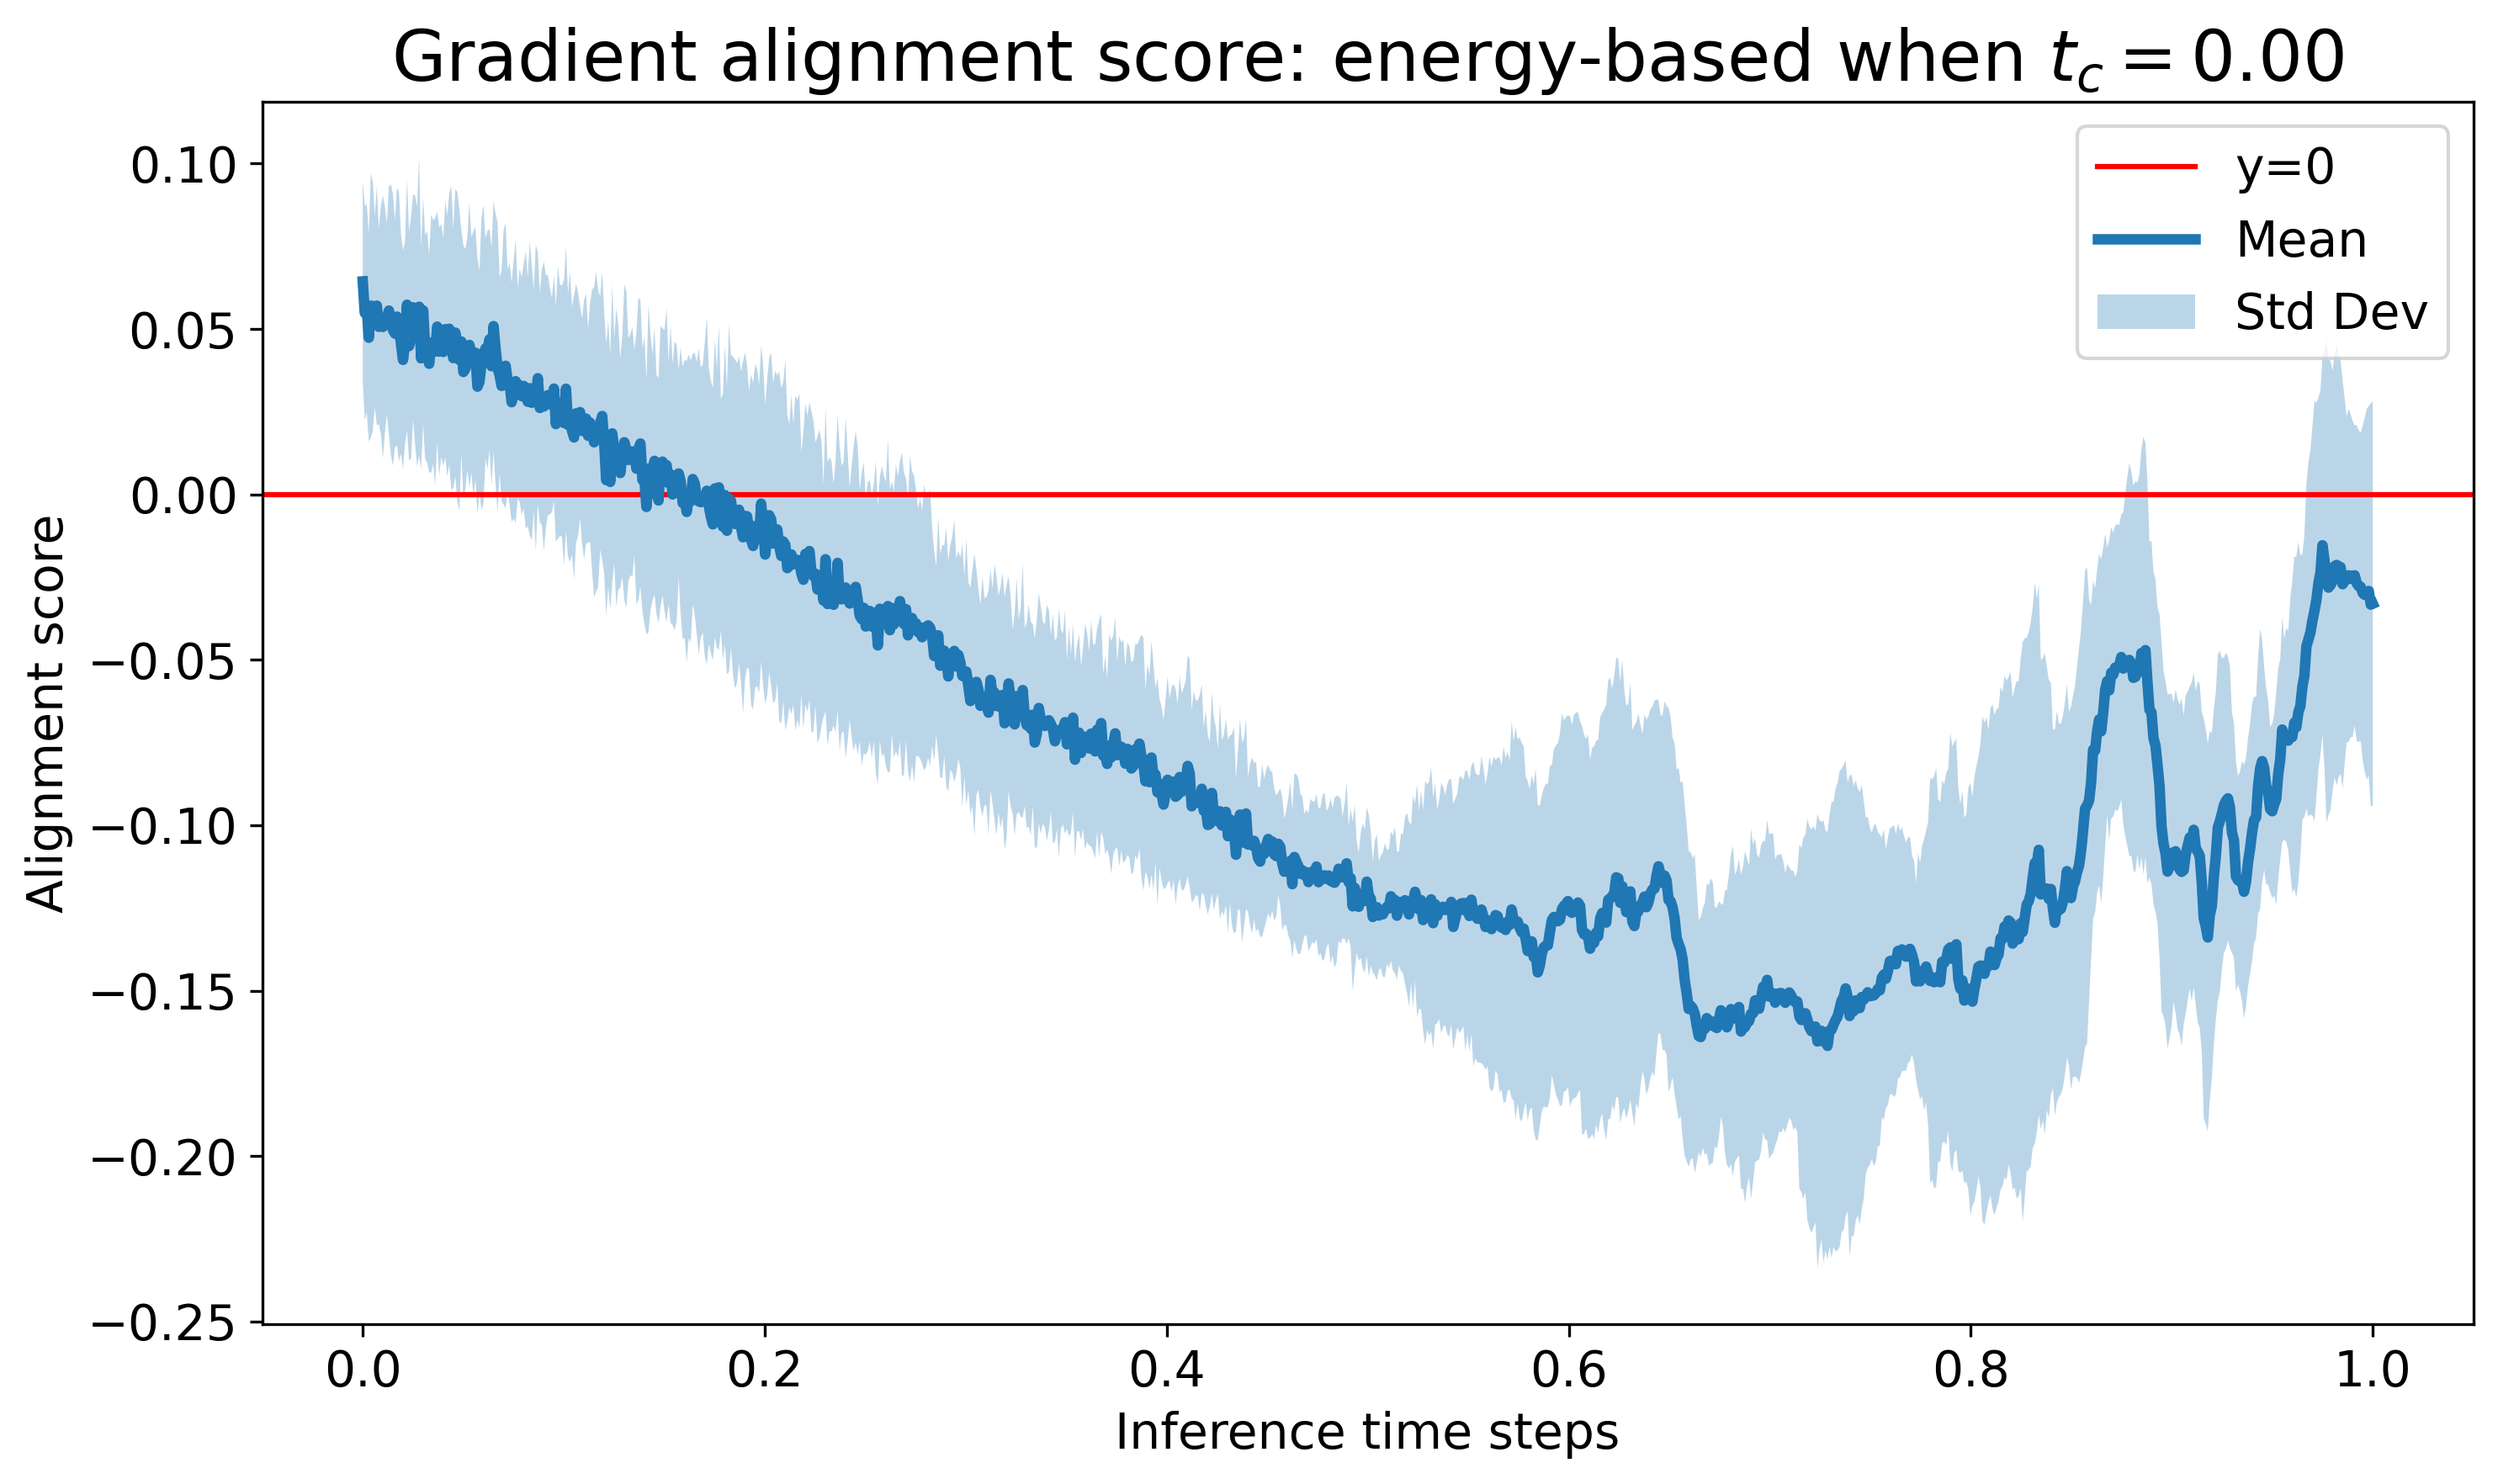
\includegraphics[width=0.8\linewidth]{chapter7/fig/mean_std_alignment_history_0.0.png}
    \caption{The gradient alignment score of energy-based approach when $t_c = 0.0$, $T=1000$.}
    \label{ch7:fig:alignmentScore}
\end{figure}

In summary, by decoupling inference from physical‐loss optimization, \textit{Dflow‐SUR} achieves gradient‐collision‐free guidance and enhanced guidance controllability, leading to several orders-of-magnitude reduction in physical loss.


\subsubsection{Surrogate model uncertainty quantification}
\label{ch7:subsect:uncertainty}
In this section, we discuss and quantify the uncertainty of the surrogate model in estimating generated samples along the trajectory. Following a previous study by Gal and Ghahramani~\cite{ai.Gal2016}, we employ Monte Carlo dropout of neurons of the surrogate model deep net with $1\%$ neuron deactivation rate. For each generated sample, we perform $20$ independent forward passes to collect $20$ predictions. We take the standard deviation of $20$ surrogate model estimations per sample for uncertainty quantification (UQ) purposes. Thus, we define UQ for each generated sample $\mathbf{x}^k$ as 
\begin{equation}
\mathrm{UQ}(\mathbf{x}^k)=\sigma(\mathbf{x}^k)=\sqrt{\frac{1}{N-1} \sum_{i=1}^N\left(f^{(i)}(\mathbf{x}^k)-\mu(\mathbf{x}^k)\right)^2},
\end{equation}
where $N=20$ is the number of stochastic forward passes, $f^{(i)}(\mathbf{x})$ is the prediction of pass $i$, $\mu(\mathbf{x})=\frac{1}{T} \sum_{i=1}^T f^{(i)}(\mathbf{x})$ is the prediction pass mean.

To assess the overall uncertainty profile of the generated designs, we plot a violin diagram of UQ values for the full batch of 200 samples. Figure~\ref{ch7:fig:uqUnconditional} shows the statistical visualization of the distribution of surrogate model UQ for generated samples along an unconditional generation trajectory (i.e., at different time steps). The red line represents the mean UQ of the surrogate model predictions for the UIUC training dataset\footnote{UIUC Airfoil Coordinates Database: \url{https://m-selig.ae.illinois.edu/ads.html} (last accessed on 23 July 2025). The database is established by the Applied Aerodynamics Group at the University of Illinois Urbana-Champaign.}. Observations reveal that during most of the early stages of the generated trajectory, the generated samples notably deviate from the mean line, indicating substantial uncertainty. Consequently, the gradients of the $\mathcal{L}_{\mathrm{phys}}$ connected to the surrogate model become inaccurate in this phase. Combined with other observations  illustrating four physics injection strategies for energy-based methods (shown in Figure~\ref{ch7:fig:uqEnergy} in Appendix~\ref{ch7:sect:AppendixUncertainty}), it remains challenging to identify an optimal physics injection time $t_c$ that balances model uncertainty while ensuring thorough optimization of the $\mathcal{L}_{\mathrm{phys}}$.

\begin{figure}[htbp]
    \centering
    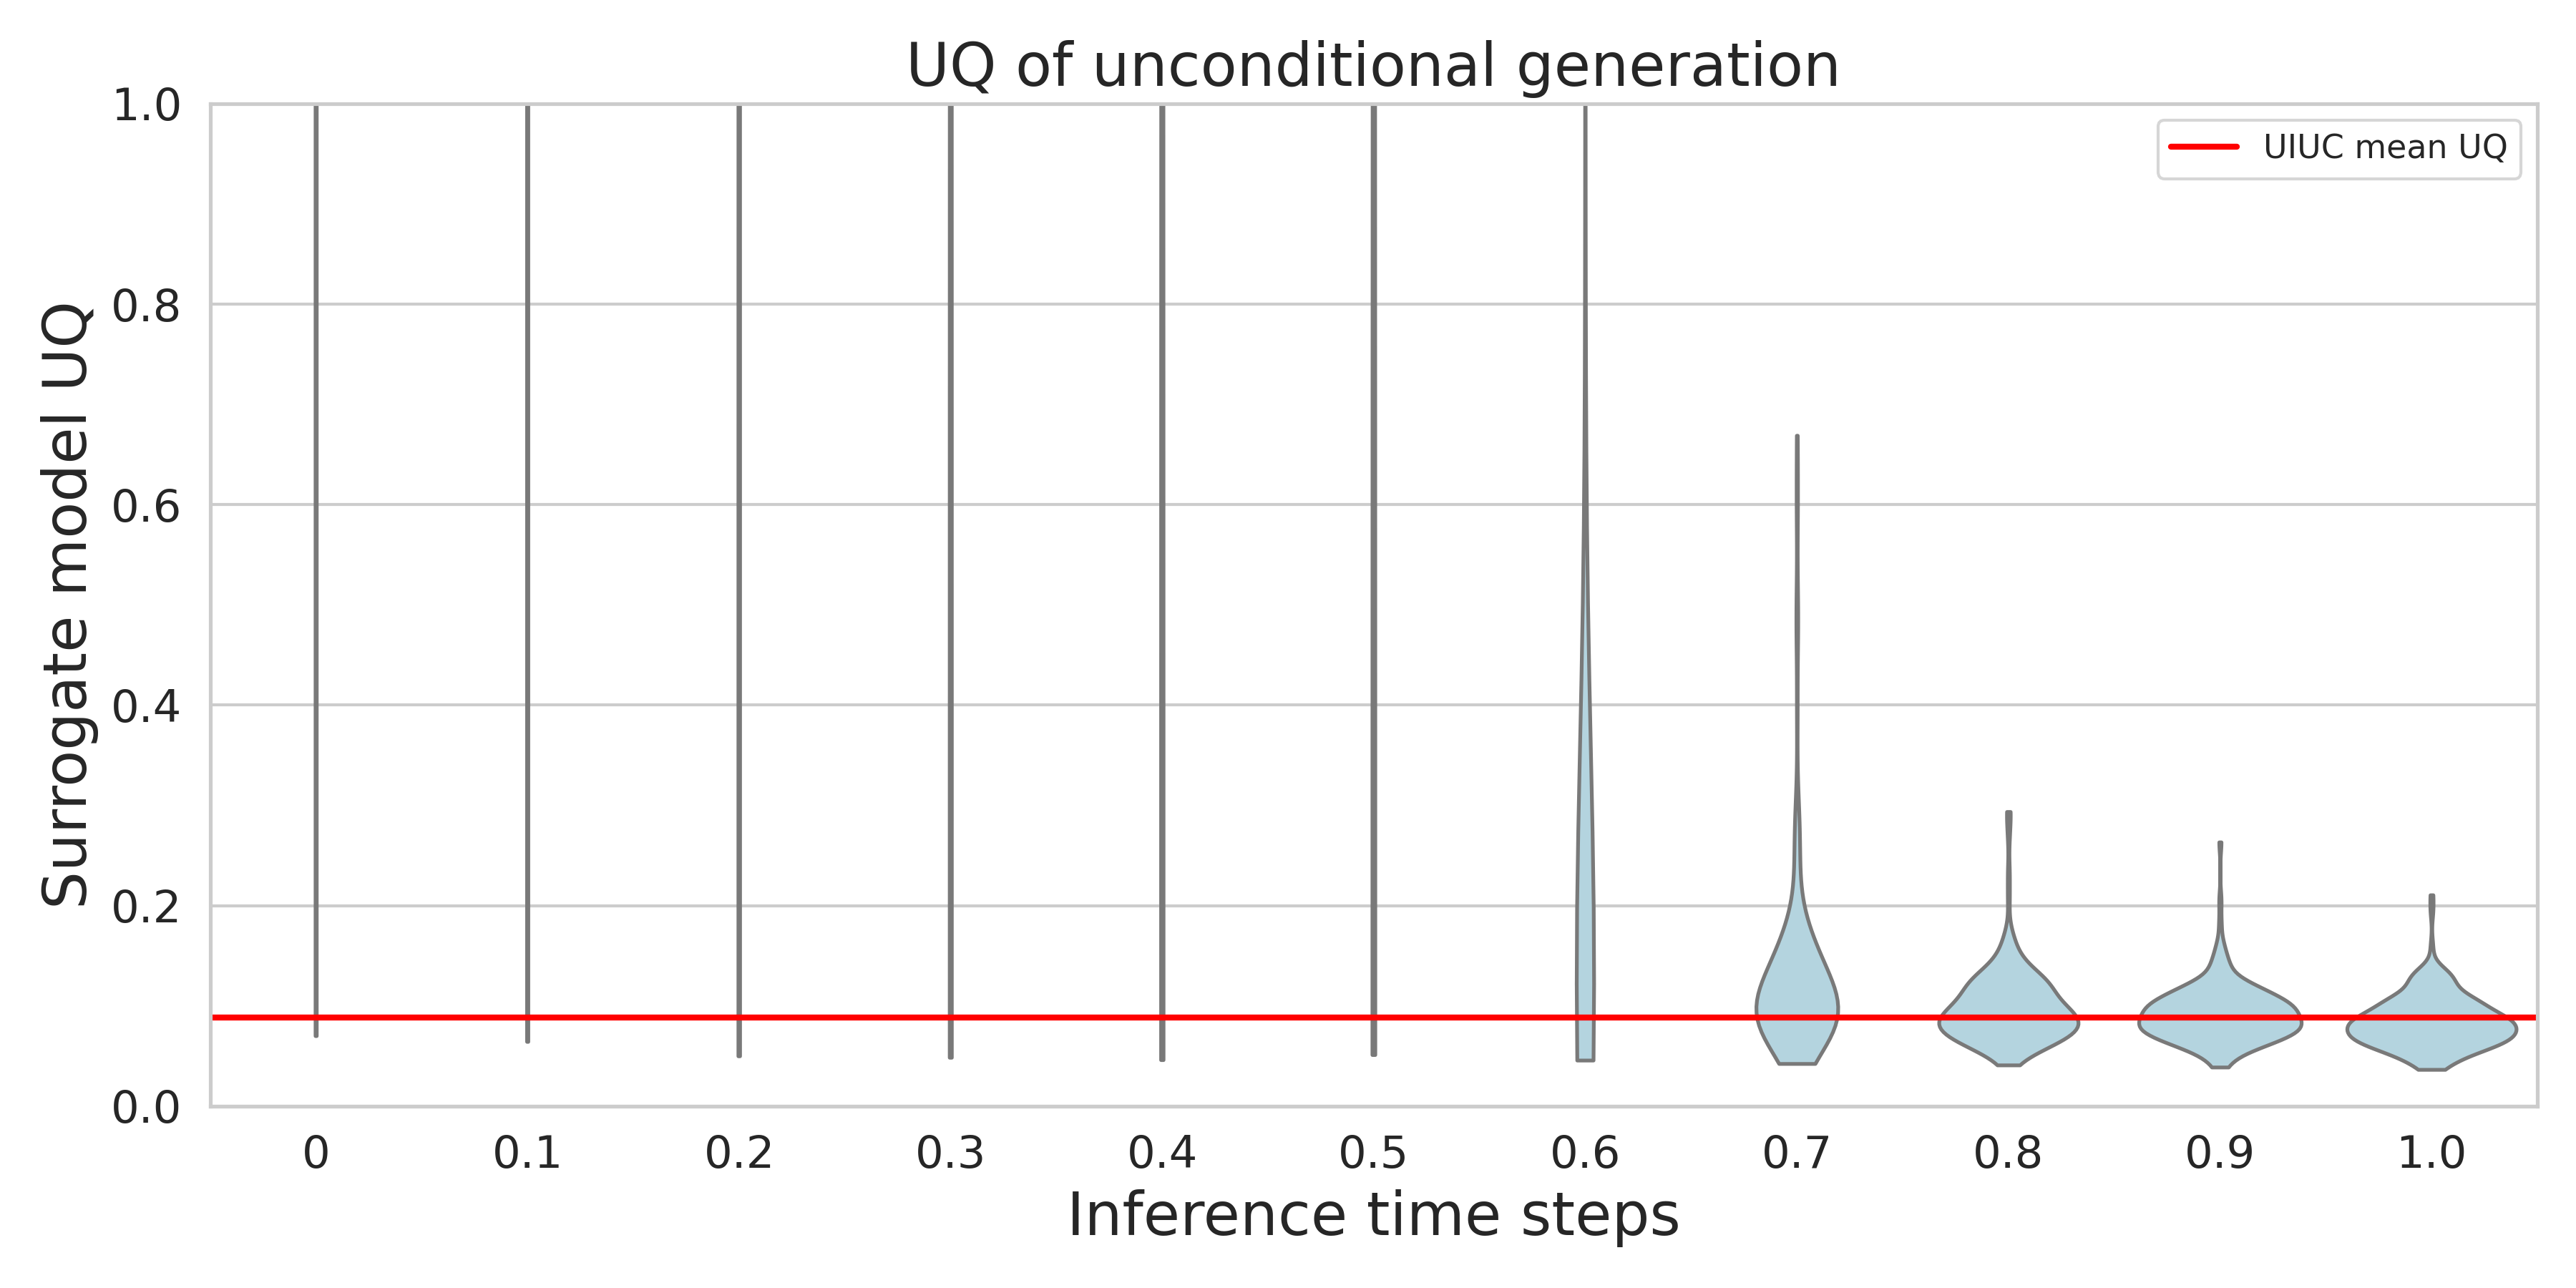
\includegraphics[width=1.0\linewidth]{chapter7/fig/UQ_uncondition.png}
    \caption{The normalized violin plot illustrates the uncertainty (UQ) of unconditionally generated samples along the denoising trajectory, with the red line indicating the mean UQ of UIUC airfoils.}
    \label{ch7:fig:uqUnconditional}
\end{figure}

Next, we show the UQ of the surrogate model for the first and final iterations generated by \textit{Dflow-SUR} in Figure~\ref{ch7:fig:uqDflowSUR}. The sample distributions of these two datasets are concentrated around the mean value (red line), thereby ensuring the stability of the surrogate model's gradients. This is formally guaranteed by Theorem 4.2 of D-Flow \cite{ai.BenHamu2024}, which ensures that the method inherently generates samples confined to the data manifold. Under the Affine Gaussian Probability Path (AGPP) (i.e., Equation 12 in Ref.~\cite{ai.Lipman2022}) assumption, they show that the Jacobian of the mapping from the noise input $\mathbf{x}_0$ to the output $\mathbf{x}_1$ is a time-ordered exponential of local covariance matrices,
\begin{equation}
D_{\mathbf{x}_0} \mathbf{x}_1=\sigma_1 \mathcal{T} \exp \left[\int_0^1 \gamma_t \operatorname{Var}_{1 \mid t}(\mathbf{x}(t)) d t\right],
\label{ch7:eqn:manifold}
\end{equation}
where $\mathcal{T} \exp [\cdot]$ stands for a time-ordered exponential and $\gamma_t$ is defined as $\gamma_t=\frac{1}{2} \frac{d}{d t} \frac{\alpha_t^2}{\sigma_t^2}$, in which $\alpha_t$ is the mean-scaling coefficient that defines AGPP and is used to interpolate between noise and data. Equation~\ref{ch7:eqn:manifold} indicates that each infinitesimal update projects the gradient onto the principal directions of data variance (i.e., the data manifold). Discretizing this ODE with \(N\) uniform Euler steps of size \(h = 1/N\) yields the Jacobian of \(\mathbf{x}_1\) with respect to \(\mathbf{x}_0\):
\begin{equation}
D_{\mathbf{x}_0}\,\mathbf{x}_1
= \prod_{m=0}^{N-1}
  \Bigl(
    (1 + h\,a_{m h})\,I
    \;+\;
    h\,\gamma_{m h}\,\operatorname{Var}_{1\mid m h}\bigl(x_{m h}\bigr)
  \Bigr).
\end{equation}
Consequently, the optimization trajectory remains confined to the data distribution by iteratively applying the above covariance‐based projections.


\begin{figure}[htbp]
    \centering
    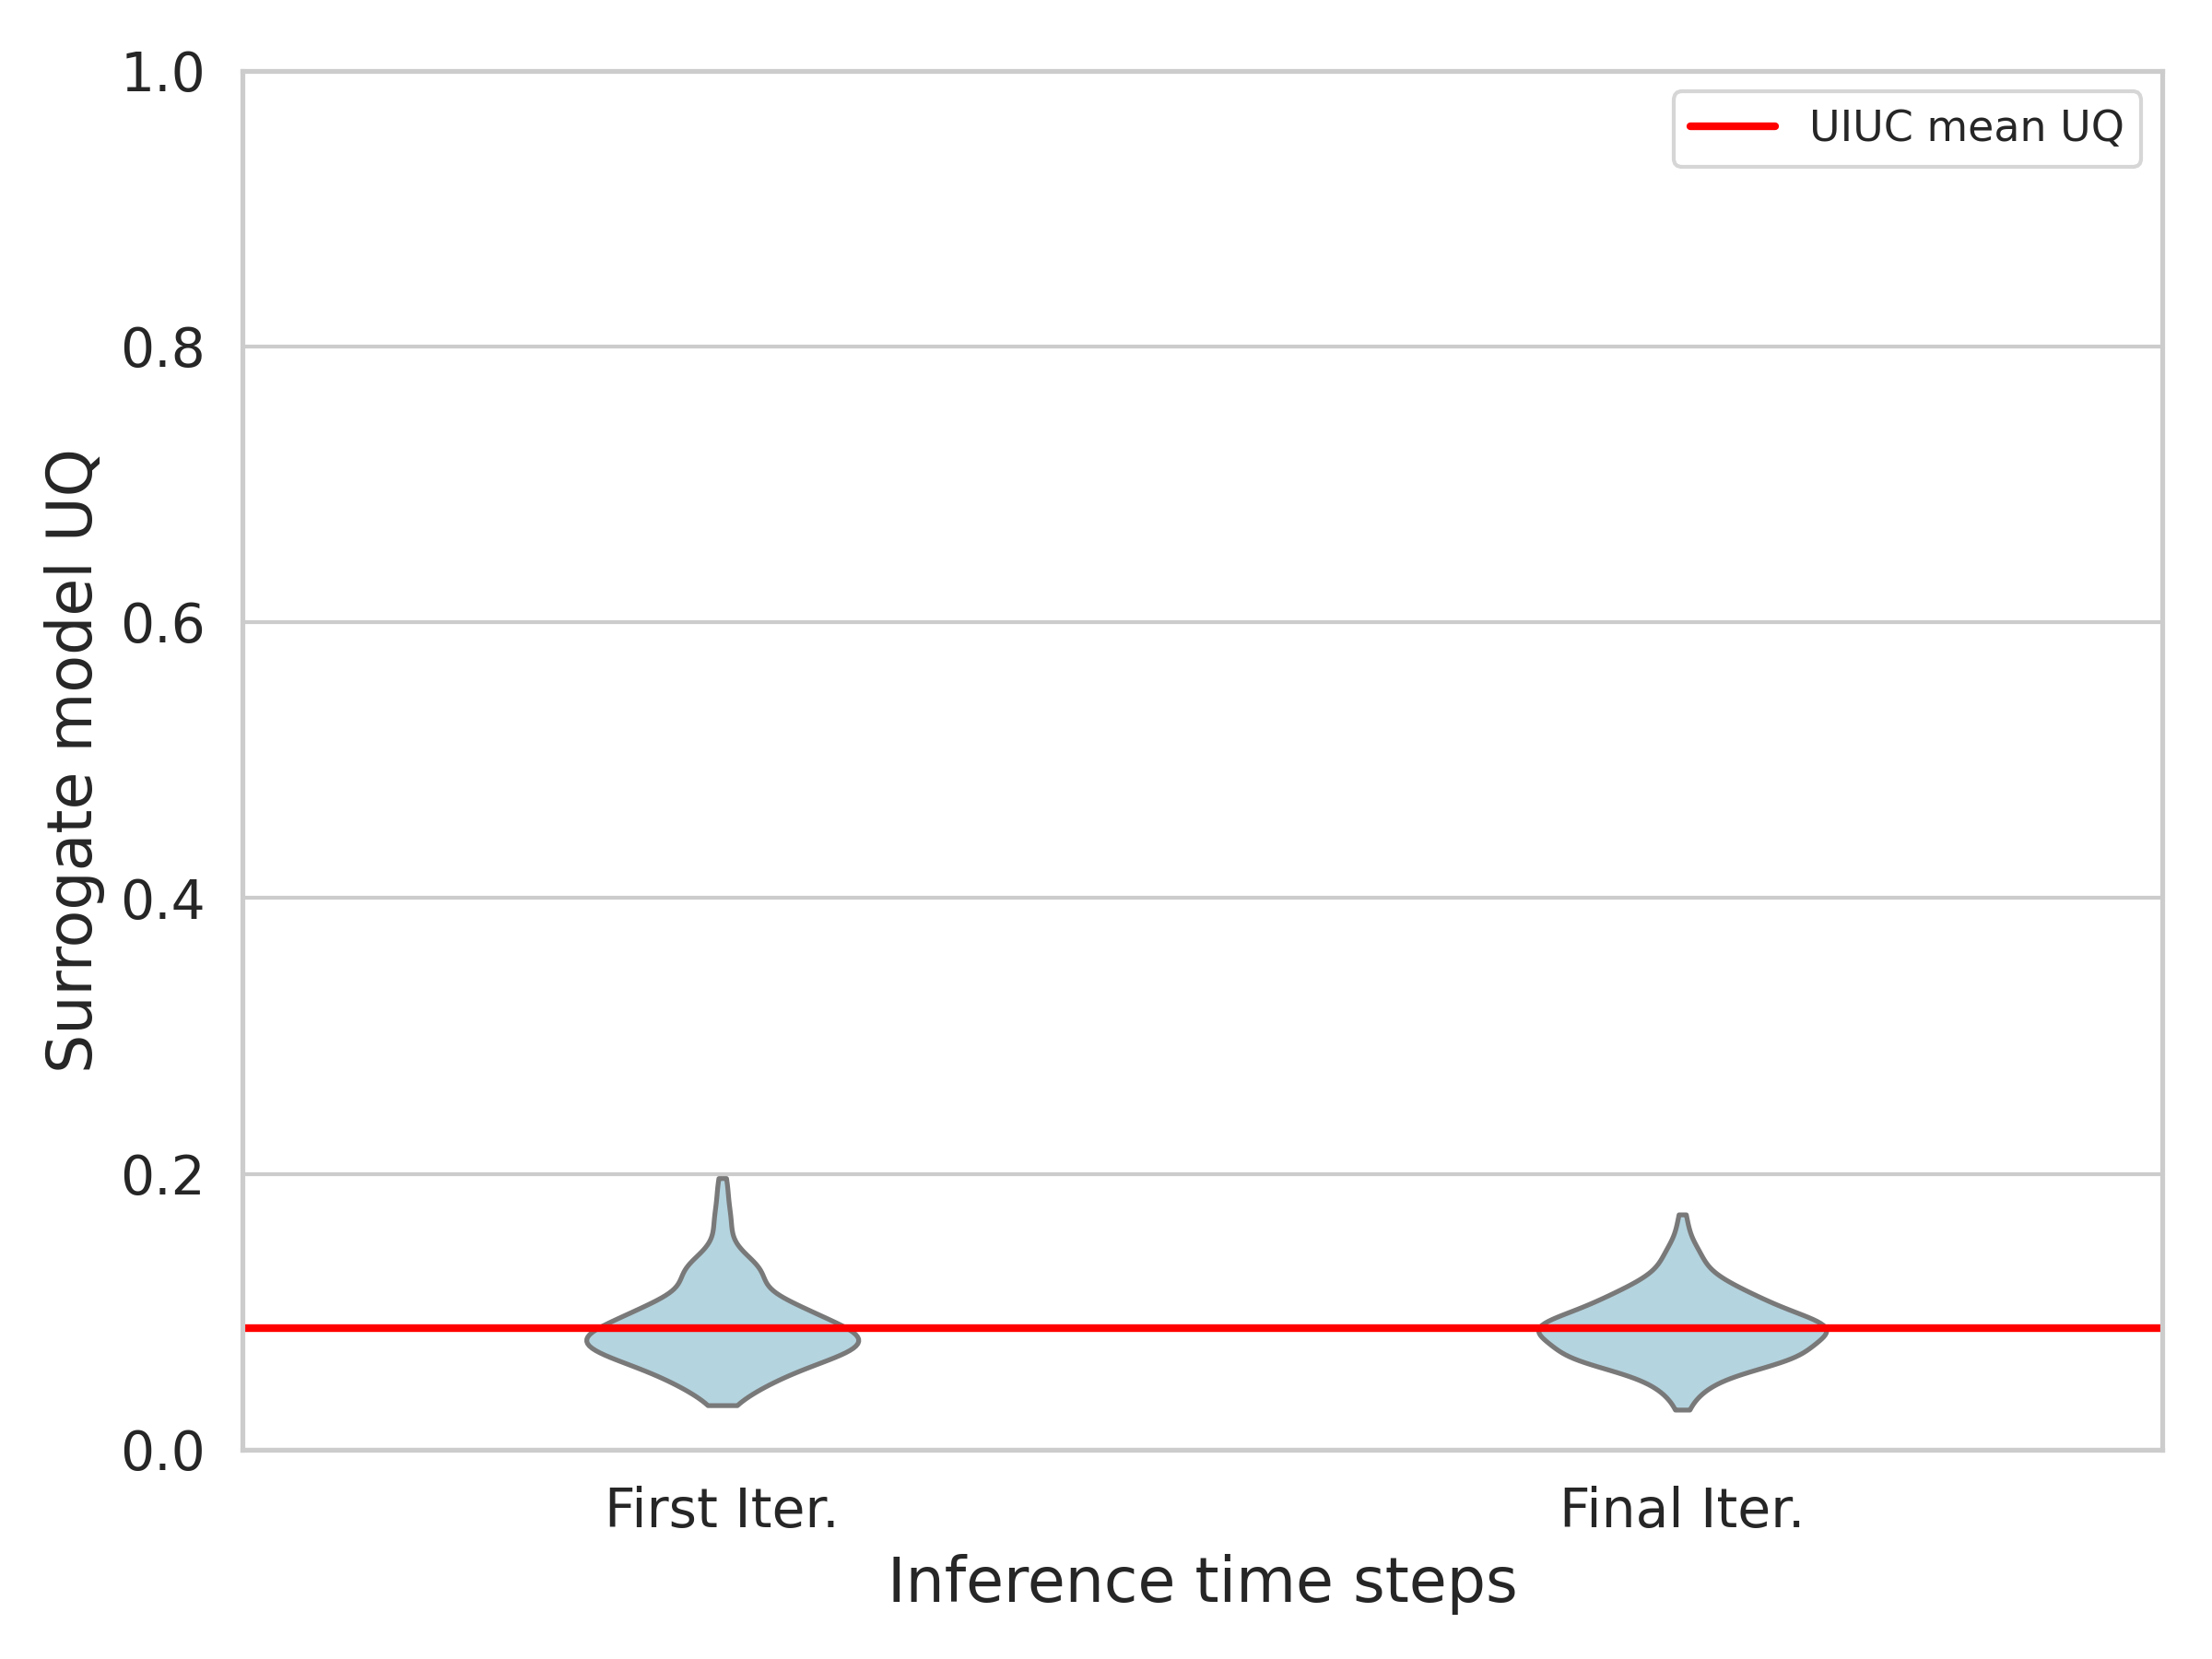
\includegraphics[width=0.8\linewidth]{chapter7/fig/dflow_uncertainty_violin.png}
    \caption{The UQ of \textit{Dflow-SUR} generates samples along the time scheduling trajectory (the red line represents the mean of UIUC airfoil UQs).}
    \label{ch7:fig:uqDflowSUR}
\end{figure}

From the above explanation, we can surmise that the energy‐based approach generates inference trajectories with large uncertainty, which undermines the surrogate model’s ability to provide reliable gradient guidance for physical‐loss optimization. In contrast, \textit{Dflow‐SUR} constrains generation along the data manifold, keeping uncertainty close to the model's mean value and avoiding manifold drifting.

\subsubsection{Sensitivity of guidance strength}
\label{ch7:subsect:diversity}
The energy-based approach requires quite a substantial manual hyperparameter tuning, which makes the process very sensitive. Table~\ref{ch7:tab:energy_diff_lambda} summarizes the experiments of energy-based approach generation with different energy coefficient $\lambda$ settings.  
\begin{table}[htbp]
    \centering
    \caption{$\mathcal{L}_{\mathrm{phys}}$ and $C_L$ for energy-based approach (when $t_c = 0.6$, T=1000) with different $\lambda$ settings.}
    \label{ch7:tab:energy_diff_lambda}
    \begin{tabular}{c c c}
        \toprule
        Energy Coefficient $\lambda$ & $\mathcal{L}_{\mathrm{phys}}$ & $C_L$ \\
        \midrule
        $1$      & $2.032 \times 10^{-2}$  & 0.565  \\
        $10$     &  $4.91 \times 10^{-4}$ & 0.706  \\
        $100$    &  $1.765 \times 10^{-4}$& 0.711\\
        $1000$   & $1.02 \times 10^{-5}$ & 0.703 \\
        $10000$  & failed & failed\\
        \bottomrule
    \end{tabular}
\end{table}
As stated in Section~\ref{ch7:subsubsect:energy}, $\lambda$ controls the energy-based approach's data exploitation and exploration. Setting this parameter either too low or too high can severely degrade the generative performance and may even cause the model to fail.

We further visualize the generated airfoils in Figure~\ref{ch7:fig:generatedAirfoil} using both the energy-based approach with various $\lambda$ and $t_c$ settings and \textit{Dflow-SUR}. 
\begin{figure}[htbp] 
    \centering
    \mbox{
        \subfloat[Energy-based: $\lambda = 0.1$, $t_c=0.0$. \label{ch7:subfig:airfoils_1}]{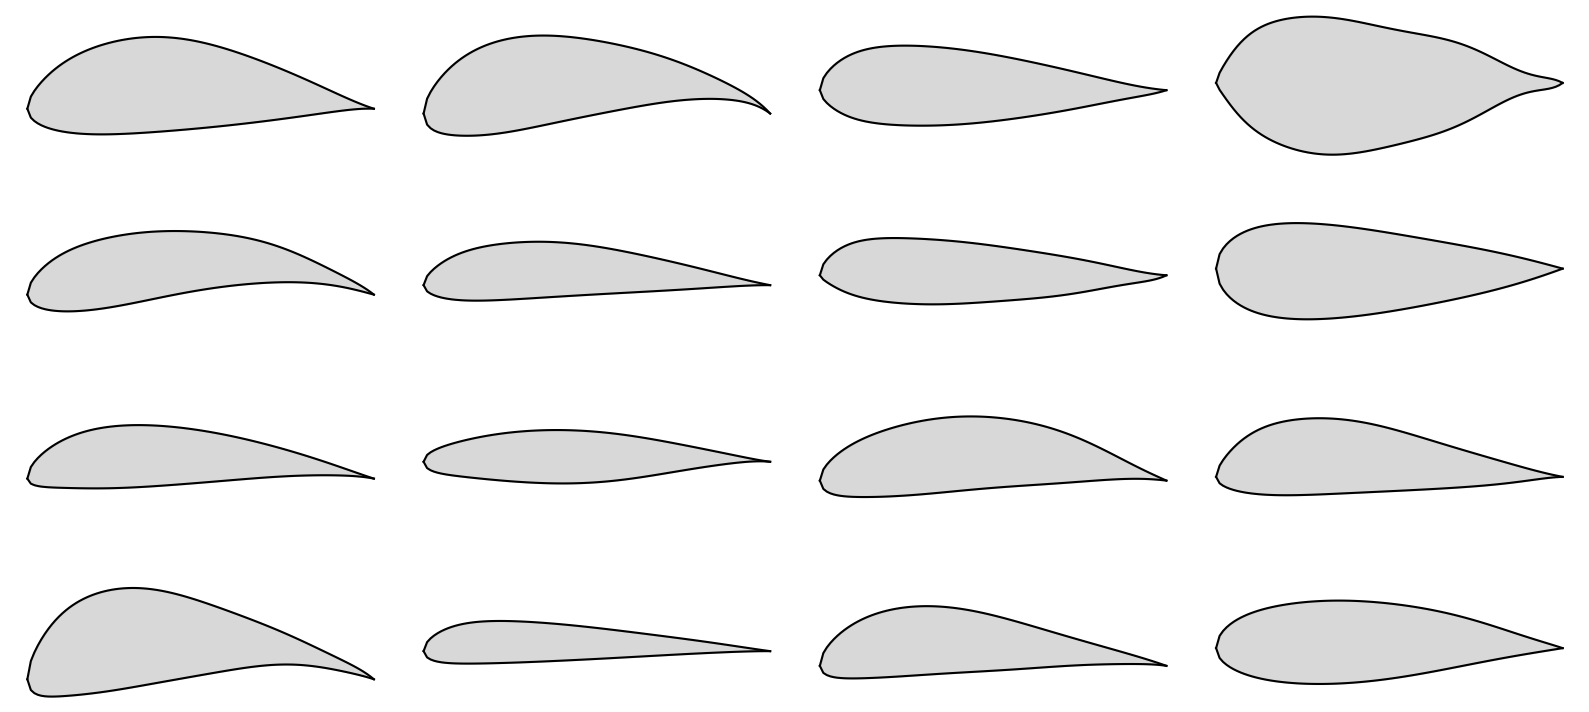
\includegraphics[width=0.4\linewidth]{chapter7/fig/lambda_0.1_tc_0.0.jpg}}
        \subfloat[Energy-based: $\lambda = 0.1$, $t_c=0.6$.]{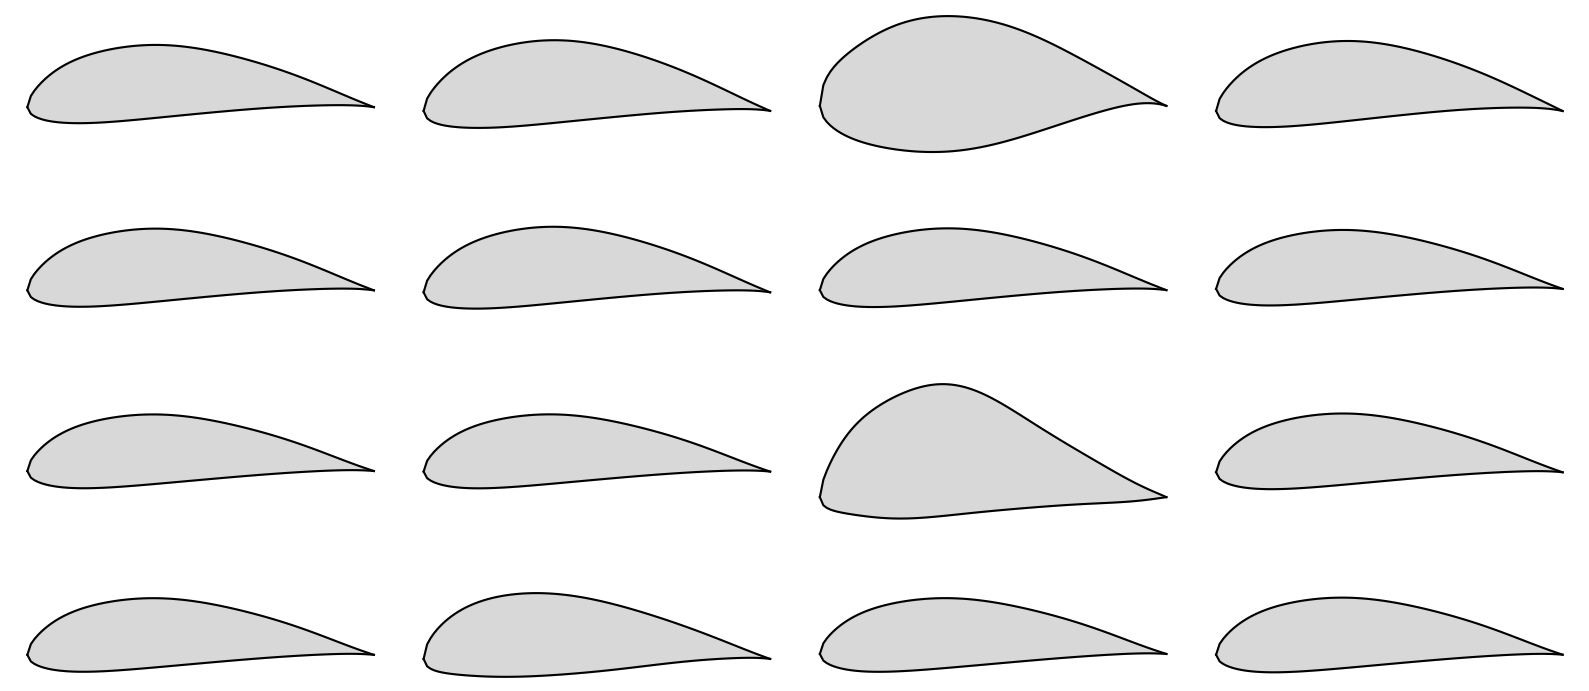
\includegraphics[width=0.4\linewidth]{chapter7/fig/lambda_0.1_tc_0.8.jpg}}
    }\\

    \mbox{
        \subfloat[Energy-based: $\lambda = 10$, $t_c=0.0$.]{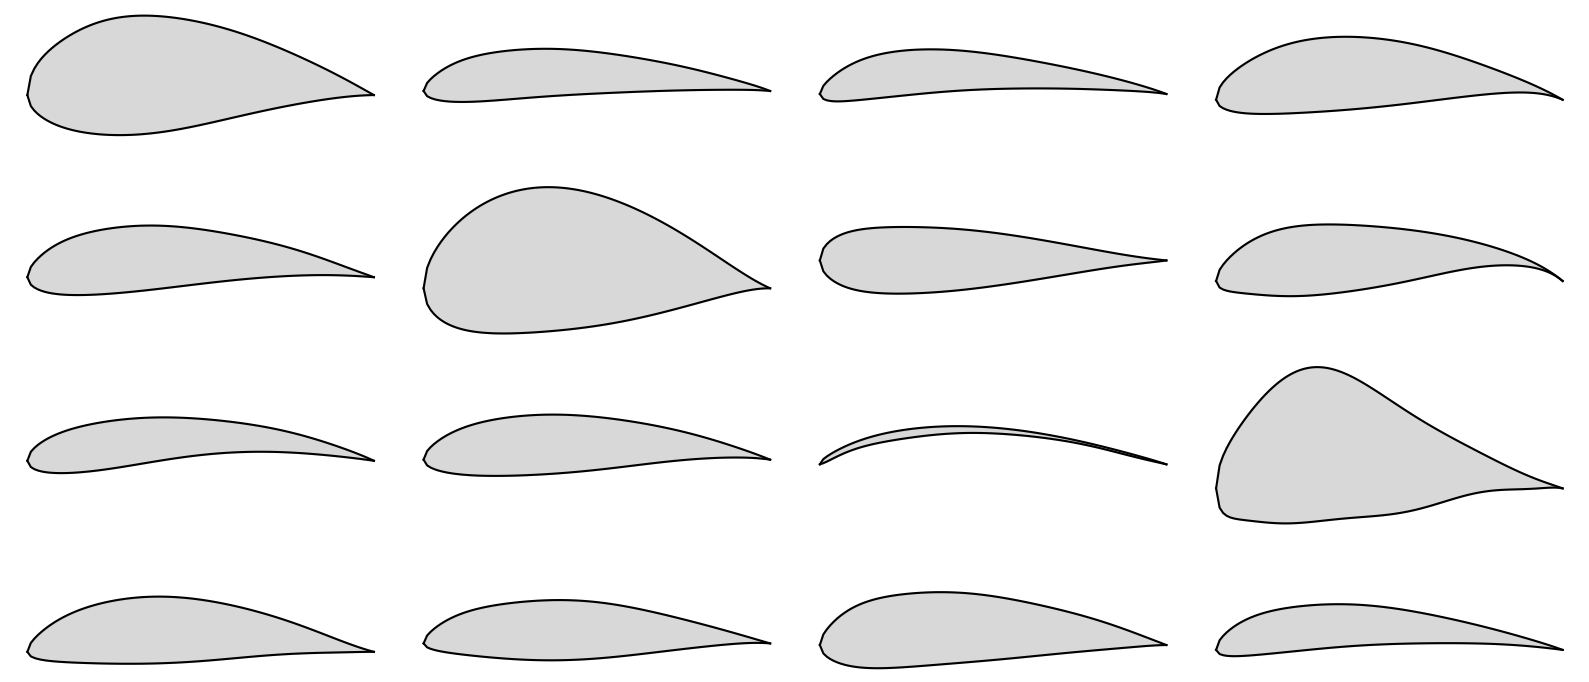
\includegraphics[width=0.4\linewidth]{chapter7/fig/lambda_10_tc_0.0.jpg}}
        \subfloat[Energy-based: $\lambda = 10$, $t_c=0.6$. \label{ch7:subfig:airfoils_4}]{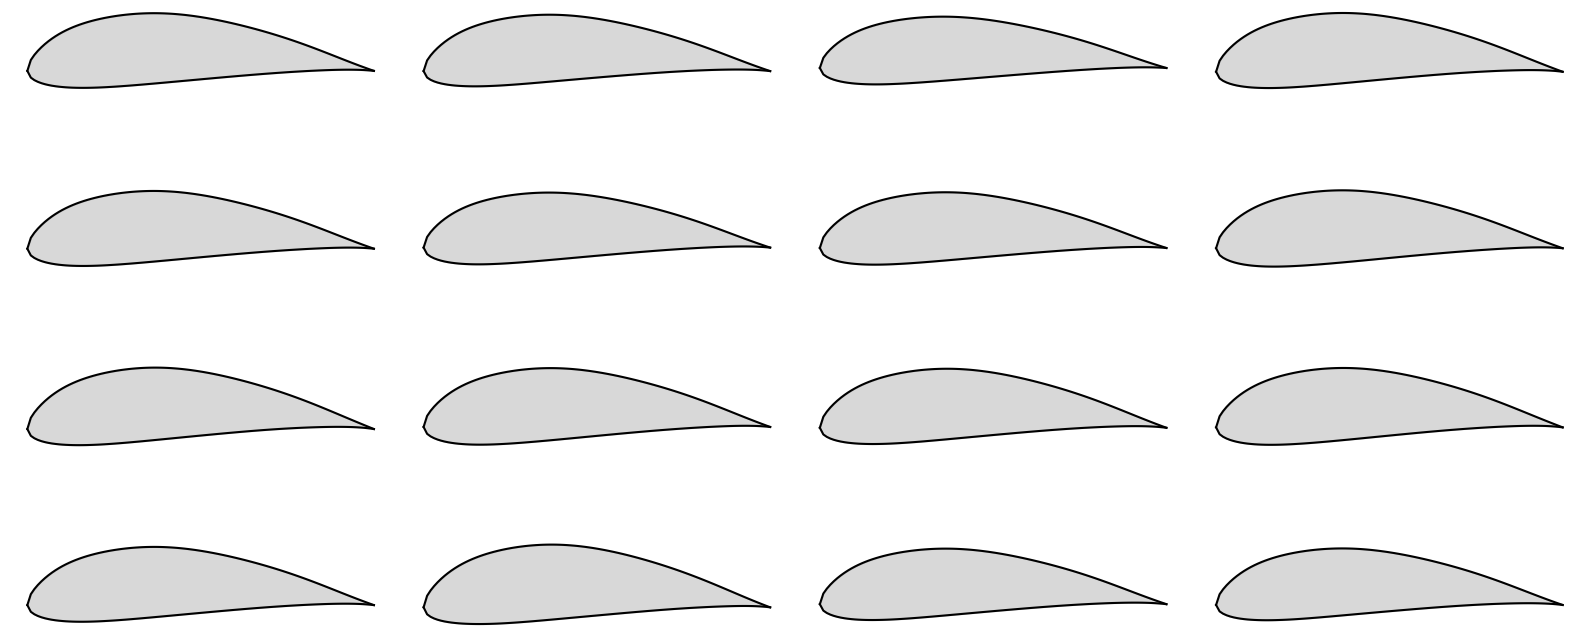
\includegraphics[width=0.4\linewidth]{chapter7/fig/lambda_10_tc_0.6.jpg}}
    }\\

    \mbox{

        \subfloat[Energy-based: $\lambda = 100$, $t_c=0.0$. \label{ch7:subfig:airfoils_3}]{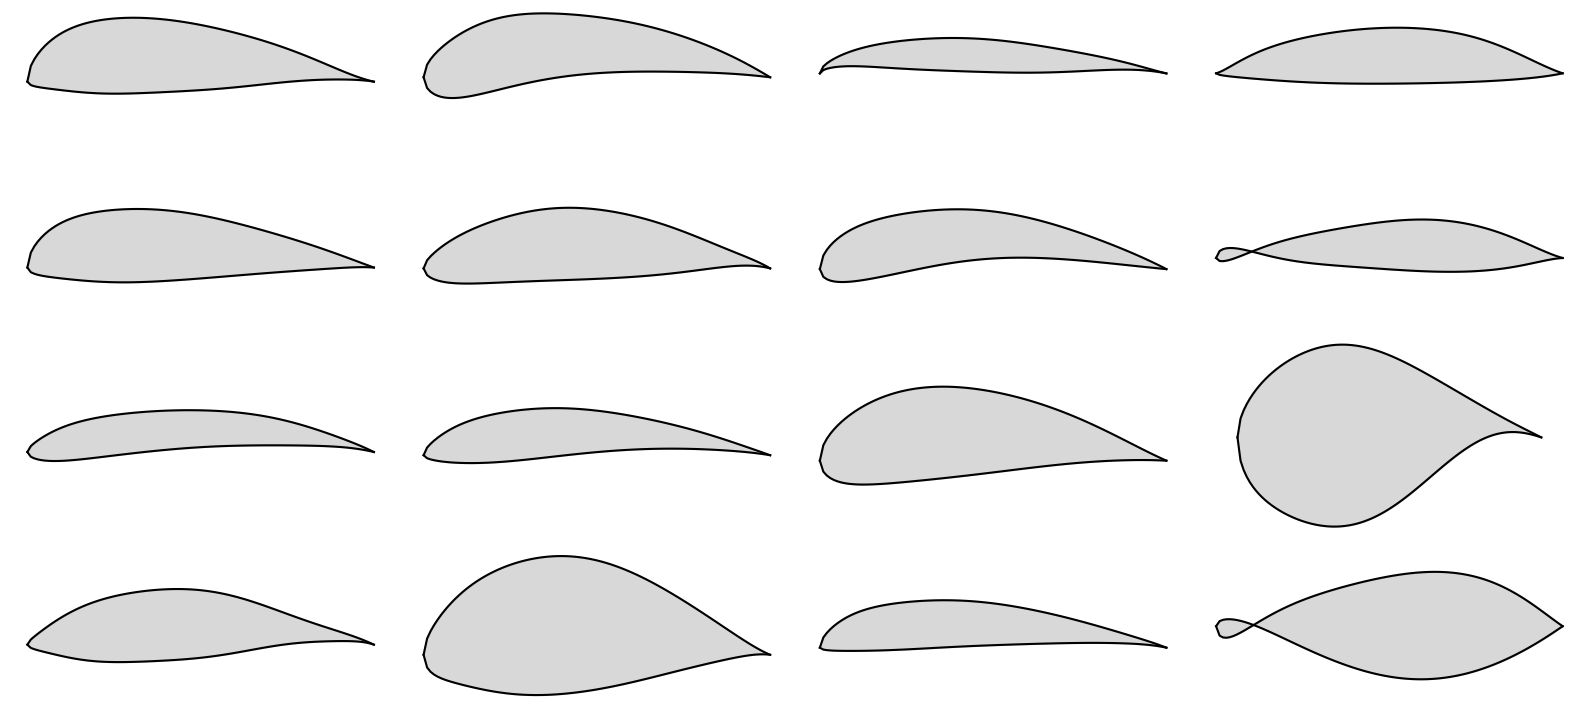
\includegraphics[width=0.4\linewidth]{chapter7/fig/lambda_100_tc_0.0.jpg}}
        \subfloat[\textit{Dflow-SUR}. \label{ch7:subfig:airfoils_6}]{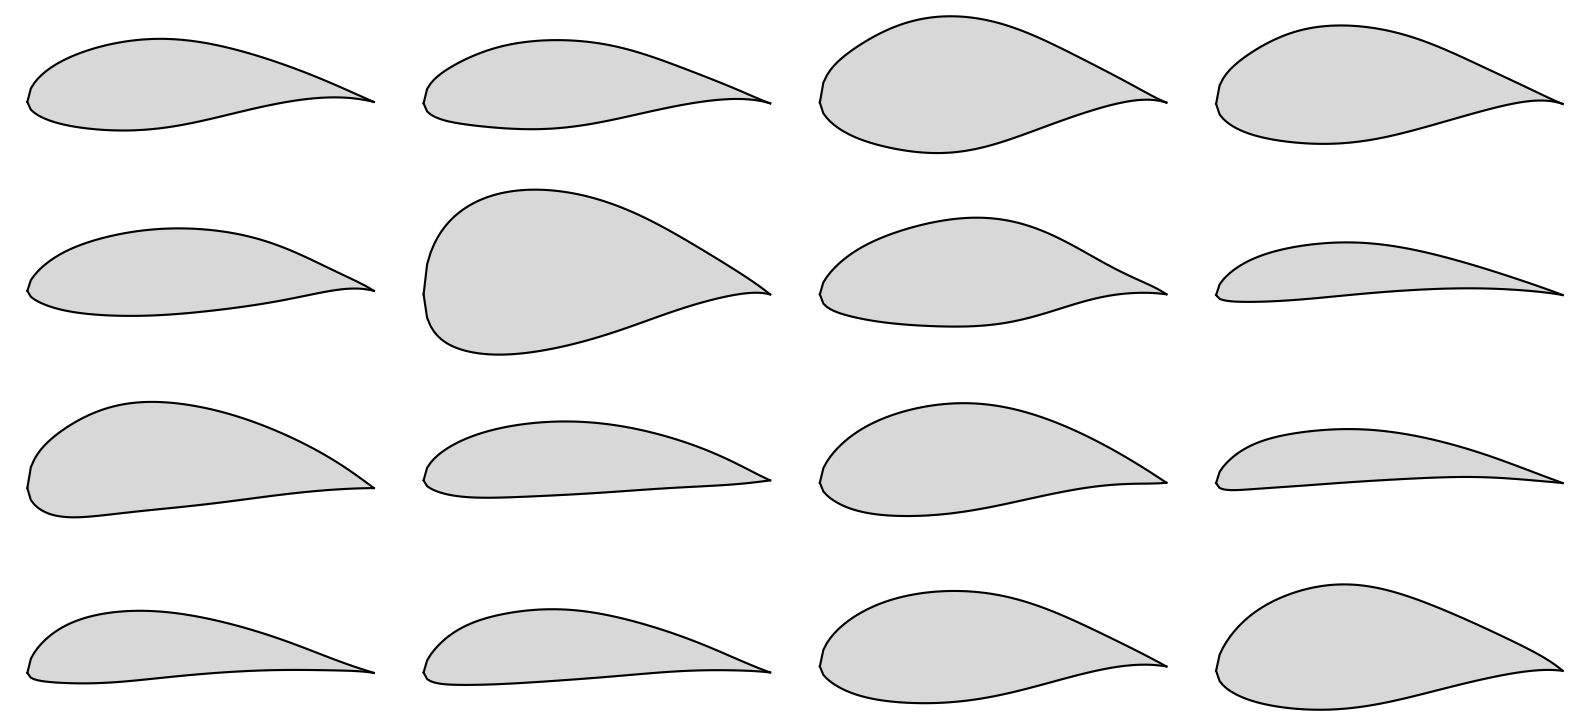
\includegraphics[width=0.4\linewidth]{chapter7/fig/dflow_SUR.jpg}}
    }
    
    \caption{Random generated airfoils using energy-based approach with various settings and \textit{Dflow-SUR}}
    \label{ch7:fig:generatedAirfoil}
\end{figure}

From the figure, we observe that using overly small or prematurely applied hyperparameters (e.g., $\lambda = 0.1$ or $t_c = 0.0$) does not degrade sample diversity but significantly increases the failure rate and fails to enforce physical constraints. Conversely, employing excessively large or belated hyperparameters (e.g., $\lambda = 100$ or $t_c = 0.8$) guarantees high-quality, constraint-satisfying outputs but sharply limits generative diversity. The samples generated by \textit{Dflow-SUR}, on the other hand, can strike the right balance between diversity, constraint satisfaction, and output quality.

In summary, the energy-based method’s sensitivity to guidance strength makes reliable generation challenging. In contrast, \textit{Dflow-SUR} requires only random initial guesses, and its decoupled execution naturally ensures both physical validity and high geometric quality of the generated samples.
